\documentclass[tikz,border=8pt]{standalone}
\usepackage{lmodern}
\usepackage{pgfplots}
\pgfplotsset{compat=1.18}
\usetikzlibrary{arrows.meta,calc,decorations.pathmorphing}
\definecolor{ink}{HTML}{183B4E}
\definecolor{teal}{HTML}{168C8C}
\definecolor{gold}{HTML}{D9982F}
\definecolor{violet}{HTML}{7B61A8}
\definecolor{softblue}{HTML}{EAF4F6}
\begin{document}
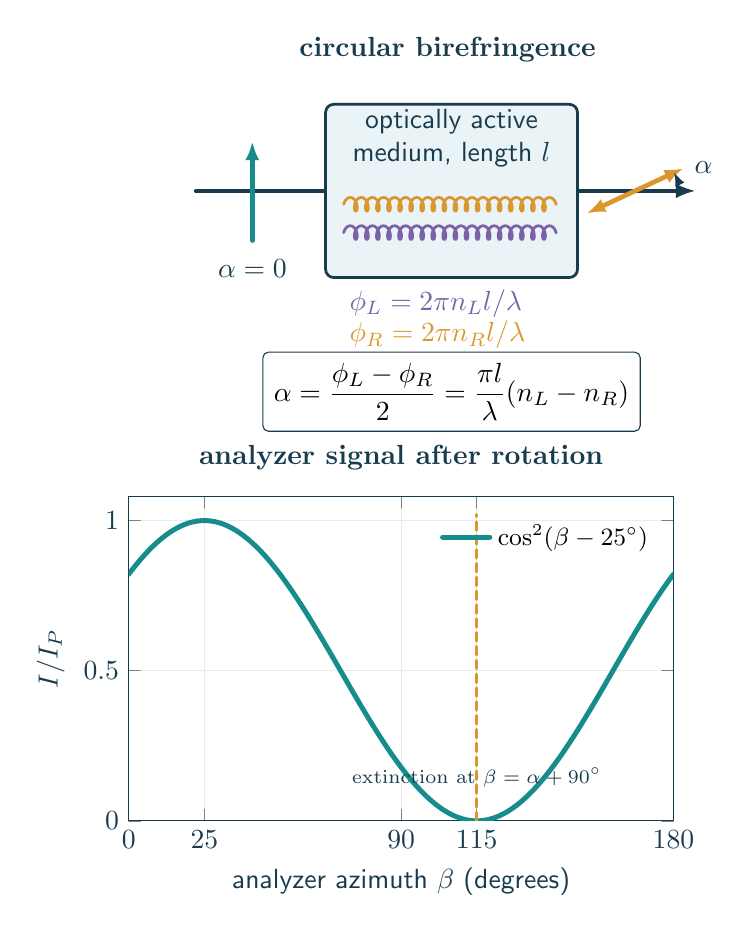
\begin{tikzpicture}[>=Latex,font=\sffamily,line cap=round,line join=round]
  % Optical-activity schematic.
  \begin{scope}[shift={(1.05,6.65)}]
    \node[ink,font=\bfseries] at (3.0,3.15) {circular birefringence};
    \draw[ink,line width=1.25pt,-{Latex[length=2.5mm]}] (-0.2,1.35)--(6.15,1.35);
    \path[draw=ink,fill=softblue,rounded corners=3pt,line width=1pt]
      (1.45,.25) rectangle (4.65,2.45);
    \node[ink,align=center] at (3.05,2.02) {optically active\\medium, length $l$};
    \draw[teal,line width=1.7pt,-{Latex[length=2.4mm]}] (.52,.72)--(.52,1.98);
    \node[ink] at (.52,.37) {$\alpha=0$};
    \draw[gold,line width=1.7pt,{Latex[length=2.4mm]}-{Latex[length=2.4mm]}]
      ({5.38-.68*cos(25)},{1.35-.68*sin(25)})--
      ({5.38+.68*cos(25)},{1.35+.68*sin(25)});
    \draw[ink,->] (5.93,1.35) arc[start angle=0,end angle=25,radius=.55];
    \node[ink] at (6.25,1.65) {$\alpha$};
    \draw[violet,decorate,decoration={coil,aspect=.55,segment length=4pt,amplitude=2.5pt},line width=1pt]
      (1.68,.82)--(4.38,.82);
    \draw[gold,decorate,decoration={coil,aspect=.55,segment length=4pt,amplitude=2.5pt},line width=1pt]
      (1.68,1.18)--(4.38,1.18);
    \node[violet,anchor=west] at (1.63,-.08) {$\phi_L=2\pi n_Ll/\lambda$};
    \node[gold,anchor=west] at (1.63,-.48) {$\phi_R=2\pi n_Rl/\lambda$};
    \node[draw=ink,fill=white,rounded corners=2pt,inner sep=4pt] at (3.05,-1.20)
      {$\displaystyle\alpha=\frac{\phi_L-\phi_R}{2}=\frac{\pi l}{\lambda}(n_L-n_R)$};
  \end{scope}

  % Equation-generated Malus curve.
  \begin{axis}[
    at={(0,0)},anchor=south west,
    width=8.5cm,height=5.7cm,
    title={analyzer signal after rotation},
    title style={ink,font=\bfseries},
    xmin=0,xmax=180,ymin=0,ymax=1.08,
    xlabel={analyzer azimuth $\beta$ (degrees)},
    ylabel={$I/I_P$},
    xtick={0,25,90,115,180},ytick={0,.5,1},
    grid=both,grid style={ink!10},
    axis line style={ink},tick label style={ink},label style={ink},
    legend style={draw=none,fill=none,font=\small,at={(.98,.95)},anchor=north east}
  ]
    \addplot[teal,line width=1.8pt,domain=0:180,samples=361]
      {cos(x-25)^2};
    \addlegendentry{$\cos^2(\beta-25^\circ)$}
    \draw[gold,densely dashed,line width=1.2pt]
      (axis cs:115,0)--(axis cs:115,1.02);
    \node[ink,font=\scriptsize,anchor=south] at (axis cs:115,.08)
      {extinction at $\beta=\alpha+90^\circ$};
  \end{axis}
\end{tikzpicture}
\end{document}
